\chapter[Self-Resonant Micro-Helix at X-band Frequencies]{Self-Resonant Micro-Helix for nano-Liter Volume Single-Crystals at X-band Frequencies.\blfootnote{A significant portion of this chapter is from J.~W.~Sidabras, J.~Duan, M.~Winkler, T.~Happe,  R.~Hussein, A.~Zouni, D.~Suter, A.~Schnegg, W.~Lubitz, E.~J.~Reijerse, Sci. Adv., 10~(5) (2019), eaay1394. and is reproduced under the CC BY-NC license.}}
\setcitestyle{citesep={,\,\thechapter.}}

For typical EPR experiments on proteins, a frozen solution of 0.1-1~mM concentration is prepared and placed in a microwave cavity. Standard sample volumes at X-band frequencies (nominally 9.5~GHz) are in the 200~$\mu$l range. However, frozen solution EPR experiments only allow the determination of the principal values of magnetic interactions at an active site, and thus provide only a limited view of the electronic structure. \cite{schweiger2001principles, goldfarb2018epr}

To resolve the full tensor magnetic interaction parameters, such as $g$-, zero field, hyperfine-, and, for nuclei with $I>1/2$, quadrupole-tensors, single-crystal EPR experiments must be performed. In combination with X-ray crystallography diffraction, the magnetic-interaction tensors obtained with EPR experiments can be directly related to the protein geometry to help identify and better understand the catalytic mechanism of the enzyme. \cite{Bowman2016, NiFeRev2007} Despite its usefulness, single-crystal EPR is rarely applied to protein systems due to challenges in growing crystals of sufficient quality and volume for these experiments. Many protein crystals used in X-ray crystallography diffraction are of dimensions in the 50--300~$\mu$m range and, as such, are too small to be studied using commercial EPR instrumentation. Crystallization methods, such as macroseeding,\cite{macroseeding} have the potential to increase the volume of the crystals, but such techniques are difficult to broadly implement. 

Currently, volume-limited crystals can only be studied using high-frequency EPR in a single-mode\cite{Hofbauer6623}, or, for continuous-wave experiments, Fabry-P\'{e}rot\cite{Klette94GHzPSI} resonators at W-band (94~GHz) or higher. Such high-frequency EPR spectrometers are not widely available and high-frequency conditions are usually unfavorable for advanced pulse experiments such as Electron Spin Echo Envelope Modulation (ESEEM) or Hyperfine Sub-level Correlation (HYSCORE) spectroscopies. \cite{pulseseq}

Unlike nuclear magnetic resonance (NMR), where all nuclei are excited and contribute to the NMR signal, hyperfine spectroscopy experiments, such as ESEEM, HYSCORE, and electron-nuclear double resonance (ENDOR), probe only the nuclei that are magnetically coupled to the paramagnetic center. Extending these experiments to single crystals not only provides the magnitude of the hyperfine- and quadrupole-tensors of ligand nuclear spins that interact with the paramagnetic centers, but also the associated angles relative to the geometry of the active site of an enzyme. Such interacting nuclei are either naturally abundant, such as $^1$H and $^{14}$N, or the catalytic cofactors must be enriched with nuclei such as $^2$H, $^{13}$C, $^{15}$N, and $^{57}$Fe, for further analysis of magnetic interaction tensors with respect to the first ligand-sphere. Furthermore, the same interaction tensors can be calculated from the molecular structure using quantum chemical calculations. \cite{NEESE2003125} These experimentally determined spectroscopic parameters can, therefore, be used to verify the adequacy of the level of theory which, in turn, gives confidence to the predicted electronic and geometric structure of the involved intermediates and transition states in the whole catalytic cycle. The groundwork for understanding the inner workings of enzymes lies in collecting as much accurate spectroscopic information as possible, including other spectroscopic and structural methods (for example, optical and vibrational spectroscopy, M{\"o}{\ss}bauer, X-ray spectroscopy, and diffraction, etc.). Every experiment contributes to the total picture and ultimately leads to a fundamental understanding of the catalytic mechanism of these enzymes.

To improve the sensitivity for studying single crystals using EPR on readily available spectrometers, typically at X-band frequencies, one must abandon the microwave cavity design and move to small-volume resonators based on lumped-circuits in the microwave frequency range. This allows the reduction of the sample volume by one order of magnitude, from 200~$\mu$l to 20~$\mu$l using a loop-gap resonator. \cite{hydehoff} Further reductions can be achieved by incorporating materials with a high dielectric constant in a standard resonator to reduce the active volume down to 1~$\mu$l. \cite{dielectricReson1,dielectricReson2,METT2019106585} For protein single-crystals one must reduce the volume even further (less than 0.03~$\mu$l), which requires radical new approaches.

\begin{figure*}[htb]
\centering
 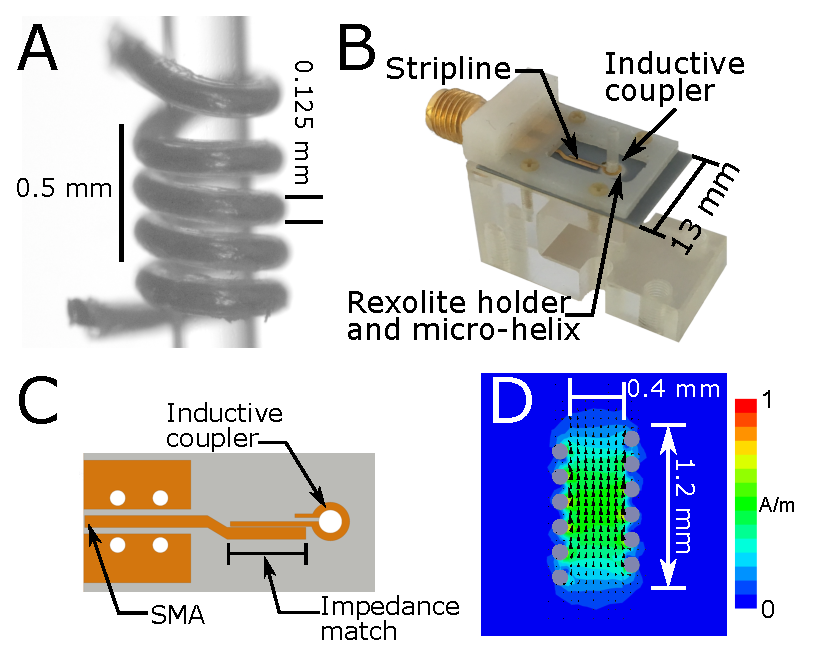
\includegraphics{Kapitel/Ch4-Images/01-MicroHelixHolder_Big2.eps}
 \caption[The self-resonant micro-helix.]{ The self-resonant micro-helix. A) A fabricated five-turn micro-helix wrapped around a 0.4~mm outer diameter capillary. The micro-helix is glued into a Rexolite holder and then placed in a B) coupling and support assembly which includes a planar micro-coupler. C) The planar micro-coupler consists of a stripline impedance-match to an inductive coupling loop. D) Finite-element modeling simulations of the microwave magnetic field normalized to Max(H$_1$).}
 \label{fig:fabricated}
\end{figure*}

The focus is on the development of resonant structures to increase EPR absolute spin sensitivity at X-band frequencies without the use of superconducting materials, which require temperatures that are sub-optimal for metallo-enzyme research and exhibit $Q$-values too large for pulse experiment, or commercial bridge modifications, which require technical expertise not commonly available in EPR laboratories. Herein, the concept of a self-resonant micro-helix, shown in Fig.~\ref{fig:fabricated}A is combined with that of a planar micro-coupler, shown in Figs.~\ref{fig:fabricated}B and \ref{fig:fabricated}C. The coupling structure on the printed circuit board is a resonant structure that drives the self-resonant micro-helix placed in the center of the coupling loop,\cite{coupling2016} shown in Fig.~\ref{fig:fabricated}B. The micro-helix geometry offers significant advantages, in that, the microwave field homogeneity is strongly improved along with volume sensitivity for small samples (Fig.~\ref{fig:fabricated}D), the microwave characteristics are optimal for pulse and continuous-wave experiments with need for very little microwave power, and the micro-helix assembly is easily matched and tuned over a variety of samples and temperatures.

In this chapter, the design and implementation of a micro-helix is outlined. Experimental and simulated comparisons of the micro-helix geometry to commercially available and state-of-the-art resonator designs are presented. To further test the micro-helix geometry two experiments were performed on photosystem II tyrosine D radical: an 85~nl frozen solution and 0.3 $\times$ 0.18 $\times$ 0.18 mm$^3$ single crystal. These data demonstrate the utility of the micro-helix in studying protein single-crystals at volumes relevant for X-ray crystallography and provide a benchmark for future work.


\section{Methods}
Four resonator geometries were compared in this work. The Bruker Biospin (i) dielectric ER4118X-MD-5W1 (MD5W1; sapphire $\epsilon_r$ of 11.5 parallel to C-axis and 9.3 perpendicular to C-axis) resonator and (ii) loop-gap resonator (LGR) ER4118X-MS-3W1 (MS3; split-ring) resonators were used as comparisons to known commercial resonator geometries. The dimensions of the MD5W1 and the MS3 can be found in Figs.~\ref{fig:geo}A and ~\ref{fig:geo}B, respectively. Additionally, two $\Omega$-shaped 0.5~mm ID planar micro-resonators (PMR) were also tested. \cite{Suter2005, Suter2008, NARKOWICZ201379, suter2015} The first PMR was printed on (iii) Rogers 6010LM (RO6010LM; Rogers Corp, Chandler, AZ, USA) substrate. The second PMR was printed on a (iv) sapphire substrate. Both PMR geometries have a 0.5~mm hole through the substrate which allows for a capillary sample to be placed in the center of the resonator. The general geometry for the PMR is shown in Fig.~\ref{fig:geo}C.

\begin{figure}[htb]
\centering
 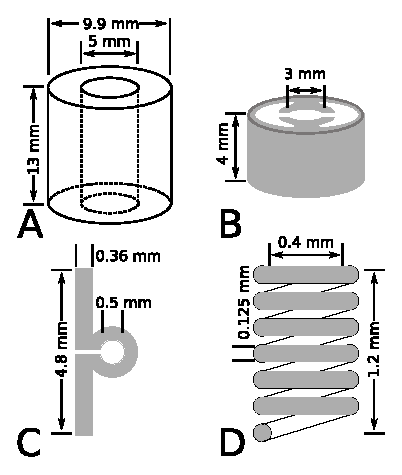
\includegraphics{Kapitel/Appendix/Images/S1-Geometries.eps}
 \caption[Geometries of resonators in this work.]{Dimensions and geometry of the four resonators compared in this work. A) Bruker Biospin ER4118X-MD-5W1 (MD5W1) sapphire dielectric resonator, B) Bruker Biospin ER4118X-MS-3W1 (MS3) split-ring resonator, C) Planar Micro Resonator 0.5~mm inner loop diameter, and D) self-resonant micro-helix with a 0.4~mm inner diameter. Grey indicates metallic surfaces.}
 \label{fig:geo}
\end{figure}

The commercially available resonators, PMR, and micro-helix designs were modeled in Ansys HFSS using driven mode. In driven mode, Ansys HFSS requires a coupling structure and mimics the output of a network analyzer. All designs are matched to 50~$\Omega$ with an S$_{11} < -35$~dB. Frequency and $Q$-values are read directly from a simulated S$_{11}$-plot and $Q_0$-values are calculated by Eqn.~\ref{q0eqn}. \cite{ginzton1957microwave} EPR signal intensity (unsaturable signal Eqn.~\ref{ch2-eq:su}; saturable signal Eqn.~\ref{ch2-eq:ss}) and resonator efficiency values (mT/W$^{1/2}$; $\Lambda_{ave}$ Eqn.~\ref{ch2-eq:lamave}) were calculated using Ansys HFSS.\cite{misrabook}  

The micro-helix is fabricated by hand winding 5 to 8 turns of 0.125~mm diameter silver wire with Polytetrafluoroethylene (PTFE) coating (0.0255~mm thickness, total 0.18~mm diameter; Science Products, GmbH, Hofheim, Germany) around a 0.4~mm drill bit and placed inside a Rexolite cylinder (0.8~mm inner diameter and 1.2~mm outer diameter) with a length of 10~mm. The drill bit was removed as the coil is affixed with super-glue by capillary action, waiting 1 minute, and blowing out the excess. The assembly was left to dry for several days. 

The coupling loop was designed in Ansys HFSS and prepared for fabrication with AutoDesk Inventor Professional 2019. The printed circuit board designs were emailed to Streamline Circuit (Santa Clara, CA, USA) engineers and manufactured on a PTFE substrate. The printed circuit board was connected to the bridge by a high-frequency SMA end launcher (AmphenolRF; 901-10510-1). Impedance matching was achieved by moving the micro-helix relative to the coupling loop until critically coupled on a network analyzer. If required, fine-tune matching is obtained with a slide-screw tuner at the bridge output. 

Bench tests of resonator characteristics, such as the frequency measurements, $Q_0$-value, and sample frequency shifts, were performed on an Agilent 8722ES (now Keysight Technologies; Santa Rosa, CA, USA) vector network analyzer.

A comparison of resonator EPR characteristics was performed on an Elexsys E580 X-band bridge by Bruker Biospin. The signal-to-noise ratio for the measured data was calculated by the ratio of the acquired signal to the standard deviation of the noise voltage, defined by
\begin{equation}
 \text{SNR}=\frac{S_{p\!-\!p}}{2\sigma_{noise}}
\end{equation}
where $S_{p\!-\!p}/2$ is the mean value of the peak-to-peak (or peak for absorption spectra) signal, and $\sigma_{noise}$ is the standard deviation of the noise. \cite{schroeder2000astronomical, oppenheim1999discrete} The standard deviation of the noise was calculated using 200 points in an off-resonance region.

The photosystem II complex sample from spinach was prepared by following the BBY method. The BBY particles were placed in a 0.4~mm outer diameter capillary with a 0.3~mm inner diameter. \cite{BBY1981} The tyrosine D (Y$_D^\bullet$) radical was generated by ambient light at room temperature for a few minutes and then rapidly frozen in liquid nitrogen. The Y$_D^\bullet$ radical is well-suited as a biological test sample since it has been extensively studied and the $g$- and hyperfine tensors are known. \cite{Hofbauer6623} Using UV-VIS spectroscopy, the number of chlorophyll molecules in the sample can be determined and, taking into account that there are approximately 250 chlorophyll molecules per photosystem II complex in spinach, the approximate number of core complexes in the active volume were calculated. Each photosystem II complex contains one Y$_D^\bullet$ radical. For the sample prepared in this work, 7.9~$\mu$M/ml of chlorophyll molecules were measured, resulting in approximately 1.6$\times10^{12}$ Y$_D^\bullet$ radicals in the 85~nl that fill the micro-helix. 

Additionally, the photosystem II core complex was extracted and purified from the thermophilic cyanobacterium {\em Thermosynechococcus elongatus} and crystallized to reach a crystal size of 0.3 $\times$ 0.18 $\times$ 0.18 mm$^3$, using the method of Athina Zouni and colleagues. \cite{KERN2005147} The crystals were gradually transferred to a cryogenic protection buffer (100~mM MES, pH 6.5, 5~mM CaCl$_2$ , 30\% (w/w) glycerol, 16\% PEG2000). The photosystem II core complex forms an asymmetric unit during crystallization and has a unit cell space group symmetry P${2_1\,2_1\,2_1}$ which copies the asymmetric unit into four sites (PDB ID: 1W5C, Ref.~[5.\kern-0.4em\citenum{KERN2005147}]) for a total of eight Y$_D^\bullet$ radicals per unit cell. From the geometry, one can calculate approximately 8.9$\times10^{12}$ Y$_D^\bullet$ radicals in the sample measured herein. The active center and the Y$_D^\bullet$ of a cyanobacterium is equivalent to that of the photosystem II from spinach. 

\section{Results and Discussion}
\subsection{Self-Resonant Micro-Helix Design}
Cavity resonators, such as the Bruker Super High-Q, are not sufficiently sensitive for extremely small samples since the very small filling factor ($\eta$ Eqn.~\ref{eq-2:filling}) is not compensated by the high $Q$-value (Eqn.~\ref{ch2-Qval}) resulting in a poor EPR signal. \cite{ReijerseSavitsky2017} Therefore, one way to maximize $\Lambda_{ave}$ of Eqn.~\ref{ch2-eq:lamave} is to reduce the size of the resonant structure relative to the sample volume, increasing the filling factor. The challenge arises due to potentially increasing the losses in the system, degrading the $Q$-value, more than the increase in the filling factor. Two common methods to reduce the size of a resonant geometry is to either use dielectric resonators (DR) to reduce the wavelength and, consequently, the size of the resonator or loop-gap resonators (LGR) to reduce the cut-off frequency of a waveguide by introducing protrusions to create regions of inductive loops and capacitive gaps. However, to study sample volumes less than 0.03~$\mu$l, further resonator reduction strategies are needed.

Limitations to minimizing LGR geometries stem from an increase in Ohmic losses due to a reduction in the gap spacing to maintain a constant resonant frequency as the sample-loop radius is reduced. In practice, this has put a limit on the $\Lambda_{ave}$ obtainable to less than 1~mT/W$^{1/2}$ for X-band frequencies. Further EPR signal improvement is possible using dielectric resonators by increasing the dielectric permittivity, and dielectric resonators with permittivity up to 80 have been used for continuous-wave EPR experiments on crystals of porous materials and polymers. \cite{dielectricReson1, dielectricReson2} However, such resonators exhibit $Q$-values over 2500 that make pulse experiments problematic. \cite{Friedlaender2015} 

Several other approaches have been followed to develop application-specific resonators for micro-samples: microstrip resonators (MR)\cite{Microstrip2009, GhirriMicroStrip}, ultra-miniature micro-resonators (UMR, 2-150 $\mu$m)\cite{AharonBlankUltra2013}, surface loop-gap micro-resonators (LGMR, 50-150 $\mu$m)\cite{AharonSurface2010}, very high-permittivity dielectric resonators \cite{walsh86, GOLOVINA200852}, and planar micro-resonators. \cite{Suter2005, Suter2008, suter2015} All of which significantly reduce the size of the resonator, but have challenges that limit the usefulness for single-crystal experiments. Herein, a new type of resonator is introduced based on a self-resonant micro-helix which is particularly useful for protein single-crystal experiments at X-band and can be used as a drop-in replacement on a standard commercial system. The self-resonant micro-helix geometry, illustrated in Fig.~\ref{fig:fabricated}, solves these challenges by providing good magnetic field homogeneity, a high-efficiency parameter, an optimum $Q$-value for both pulse and continuous-wave EPR experiments, straight-forward impedance matching, and ease of sample placement. 

Helical resonators were first introduced to EPR in the early-1960s as a method to increase the microwave magnetic field at the sample. Resonant helical geometries were affixed to one end of a shorted waveguide creating a slow-wave structure. \cite{Webb1962, Helix1967} Coupling was achieved by direct connection to a coaxial line with a capacitive matching network or by microwave incident on the helical structure from a waveguide. The sample was placed within the helix and showed a reasonable sensitivity increase and larger microwave magnetic field due to higher filling factors compared to typical cavities. \cite{Nolle1966} Broadband slow-wave helical resonators were employed for multi-frequency experiments, where a non-resonant structure, having a $Q$-value close to unity, could be matched with a slide-screw tuner over an octave bandwidth. \cite{nonresonant1986} However, over time, they were replaced by loop-gap resonators which achieved higher concentration sensitivity for limited samples. \cite{froncisz1982loop}

Recently, micro-coils have gained popularity in NMR for nano-liter samples \cite{Olson1967, SUBRAMANIAN1998227, cr980140f,Kentgens2008,Raluca2011,Jones2012} and for microfluidics. \cite{Mompean2018} However, three characteristics differentiate our micro-helix configuration from those described in the EPR \cite{Webb1962, Helix1967, oldmicro} and NMR literature\cite{WEBB2005892}: (i) the helix is self-resonant, meaning that the self-inductance of $n$-turns ($L_{tot}$) and self-capacitance between the loops ($C_{tot}$) resonate at a frequency determined by $\omega^2 L_{tot}C_{tot}=1$, where $\omega$ is the resonant frequency in radians/s. Since the geometry is self-resonant, no additional capacitors are needed. A self-resonant micro-helix has lower Ohmic loss, which provides a higher $Q$-value than is typically feasible with micro-coil geometries in NMR, where, with an NMR micro-coil, a typical $Q$-value is around 30. \cite{WEBB2005892} With a self-resonant micro-helix, the volume to surface ratio is maximized and a $Q$-value of 300 is achievable. (ii) Compared to previous EPR literature, the helix length is much smaller than the wavelength (31.6~mm at 9.5~GHz), which increases the uniformity and the inner diameter is 0.4~mm at X-band frequencies, which increases the resonator efficiency. With this geometry, the micro-helix is not a slow-wave structure but an inductor at self-resonance. The normalized microwave magnetic field profile is shown in Fig.~\ref{fig:fabricated}D. (iii) Finally, the helix is coupled to an inductive coupling loop on a printed-circuit board by mutual inductance, which can be designed to minimize noise and further increase the EPR signal-to-noise ratio. \cite{coupling2016} Mutual inductance coupling does not require a balun or capacitive matching network, simplifying coupling methods.

\subsection{Simulated Comparison of a Planar micro-resonator \& a self-resonant micro-Helix} 

\begin{wrapfigure}{L}{3.5cm}
\centering
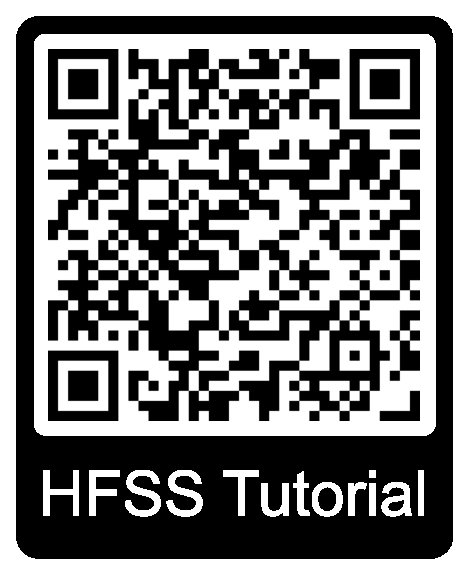
\includegraphics[width=3.5cm]{Kapitel/Appendix/HFSSTutQR.eps}
\end{wrapfigure}

In this section an eigenmode solution is constructed for both the PMR and micro-helix to compare how the signal (Eqns.~\ref{ch2-eq:ss} and \ref{ch2-eq:su}) and resonator efficiency $\Lambda_{ave}$ (Eqn.~\ref{ch2-eq:lamave}) scale with a lossy aqueous sample ($\epsilon_r = 63 - i26.46$ from Ref.~[5.\kern-0.4em\citenum{EllisonWater2017}]) and relatively-lossless ice sample ($\epsilon_r=3.17-i0.0035$ from Ref.~[5.\kern-0.4em\citenum{icedielectric}]). An eigenmode solution is used for simplicity and requires no matching network. Once a micro-helix design has been chosen, a matching network is added to the structure and the resonator microwave magnetic field is directly compared at a normalized input voltage. 

The Ansys HFSS solutions are created using local variables for performing parametric sweeps.\footnote{The files can be found at \textit{https://github.com/jsidabras/HFSSTutorial} and the Ansys \textit{aedt} file has 4 projects to be solved.} For instance, the sample radius on both geometries can be varied and this parameter will be used in this comparison. Mesh operations have been added on the quartz capillary tube and on the surface of the main resonator geometry to reduce numerical fluctuations and obtain a field profile void of discontinuities. 

\begin{figure}[ht]
 \centering
 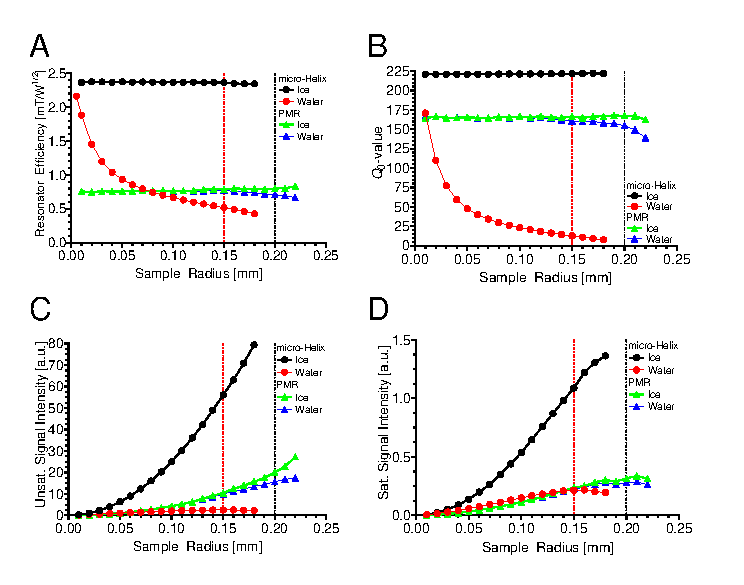
\includegraphics[width=\textwidth]{Kapitel/Ch2-Images/Ch2-SweepOutputA.eps}
 \caption[EPR characteristics as the sample radius is swept.]{EPR characteristics for the PMR with sapphire substrate (black; $\blacktriangle$) and the 0.4~mm micro-helix (red; $\CIRCLE$) with a water (solid) and ice (dashed) sample. Shown are the EPR characteristics as the sample radius is swept for the A) resonator efficiency $\Lambda_{ave}$, B) $Q_0$-value, C) unsaturated EPR signal, and D) saturable EPR signal. The dashed-dot lines indicate the largest practical capillary inner radius for the helix (red) and PMR (black).}
 \label{fig:SweptData}
\end{figure}

Shown in Fig.~\ref{fig:SweptData} are the simulated EPR characteristics for the micro-helix (red; $\CIRCLE$) and planar micro-resonator (black; $\blacktriangle$) geometries. The ice sample is shown as a dashed line, while the aqueous sample is shown as a solid line. The sample radius is swept and a quartz sample holder with a wall thickness of 0.025~mm is used. The dashed-dot line indicates the largest commercially available practical capillary inner radius for the helix (red) and PMR (black). In this study, a ``concentration sensitivity'' comparison is made where the resonator performance is evaluated assuming a varying sample volume at a fixed concentration.

\begin{figure}[htb]
 \centering
 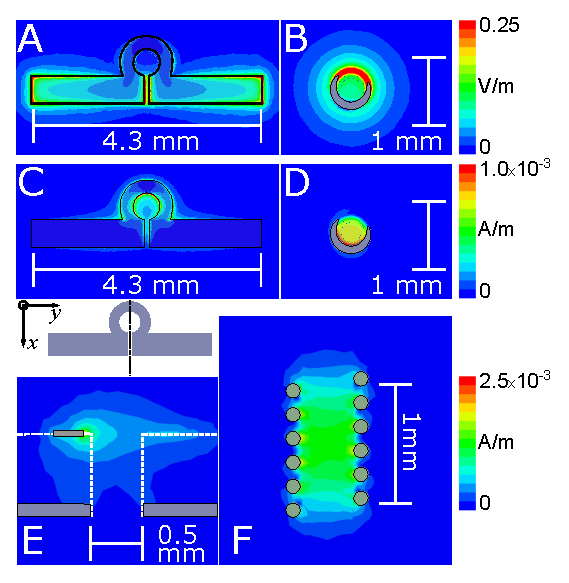
\includegraphics[width=0.9\textwidth]{Kapitel/Ch2-Images/Ch2-AnsysFields.eps}
 \caption[Simulated field distribution for Helix and PMR.]{Simulated field distribution for the magnitude of the electric field for the A) planar micro-resonant (PMR) and B) micro-helix and the magnitude of $\mathbf{H}_{1r}$ with $\mathbf{H}_0$ in the $y$-direction for the C) PMR and D) micro-helix in the $x$-$y$-plane. And the magnitude of $\mathbf{H}_{1r}$ with $\mathbf{H}_0$ in the $y$-direction for the E) PMR and F) micro-helix in the $x$-$z$-plane with a normalized voltage input. }
 \label{ch2-fig:FieldData}
\end{figure}

For the PMR (black; $\blacktriangle$), little change in both the average resonator efficiency $\Lambda_{ave}$ and $Q_0$-value is exhibited as the sample radius is increased, Figs.~\ref{fig:SweptData}A and \ref{fig:SweptData}B, respectively. From the simulations, the electric field (which gives rise to losses) is well contained in the planar micro-resonator geometry away from the sample loop. Shown in Fig.~\ref{ch2-fig:FieldData}A is a plot of the magnitude of the electric field. A potential is formed across the PMR gap and a gradient of charge is formed in the loop which goes to zero opposite of the gap. This is similar to the electric field profile of a one-loop--one-gap loop-gap resonator.

In the PMR, the value of $\Lambda_{ave}$ is approximately one-third of the micro-Helix (red $\CIRCLE$; in Fig.~\ref{fig:SweptData}A). The reduction in $\Lambda_{ave}$ is due to a significant portion of the magnetic field stored energy being located outside of the sample volume in the PMR geometry and significant inhomogeneity of the magnetic field along the axis. This is illustrated in Fig.~\ref{ch2-fig:FieldData}C where the magnitude of $\mathbf{H}_{1r}$ with $\mathbf{H}_0$ in the $y$-direction is plotted. A significant portion of this magnetic field lies outside of the sample region. This is also true along the axis, shown in Fig.~\ref{ch2-fig:FieldData}E, where a large gradient of $\mathbf{H}_{1r}$ is present. 

With the micro-helix geometry, the $\mathbf{H}_{1r}$ is concentrated in the center and a very little magnetic field is found outside of the sample volume, shown in Fig.~\ref{ch2-fig:FieldData}D. Additionally, the $\mathbf{H}_{1r}$ field profile along the axis is more homogeneous compared to the PMR, shown in  Fig.~\ref{ch2-fig:FieldData}F. Normalized $\mathbf{H}_{1r}$ squared, which is proportional to signal, on-axis for both the PMR (dashed) and micro-helix (solid) is plotted in Fig.~\ref{fig:HFSS}.  The homogeneous magnetic field in the micro-helix leads to a higher filling factor $\eta$ and, ultimately, a higher average resonator efficiency $\Lambda_{ave}$, as shown in Fig.~\ref{fig:SweptData}A. 

\begin{figure}[ht]
 \centering
 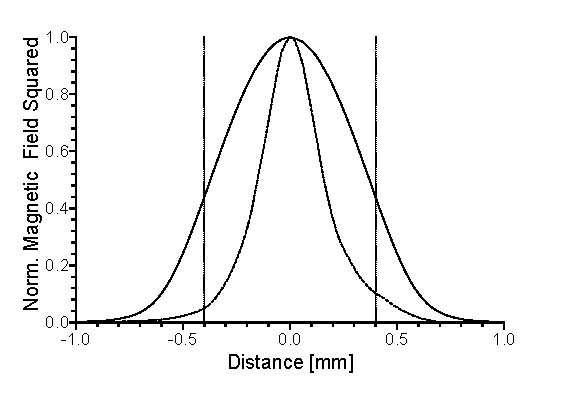
\includegraphics{Kapitel/Ch5-Images/B2OnAxis.eps}
 \caption[Magnetic Field Squared on axis: PMR vs micro-Helix.]{Magnetic Field Squared on axis of the micro-helix (solid) and PMR  (dashed) is plotted.}
 \label{fig:HFSS}
\end{figure}

As anticipated from Eqn.~\ref{ch2-eq:su}, relatively lossless samples will display EPR unsaturable signal growth that is proportional to the magnetic field squared within the sample volume, shown in Fig.~\ref{fig:SweptData}C as a dashed line for the micro-helix (red; $\CIRCLE$) and PMR (black; $\blacktriangle$). With such samples, the EPR signal expected by using the micro-helix is significantly enhanced compared to the PMR. In contrast, the saturable sample defined by  Eqn.~\ref{ch2-eq:ss} has a maximum due to the interplay of the power loss $P_l$ and the magnetic field in the sample. Since the micro-helix exhibits an azimuthal component of the electric field that penetrates the sample, shown in Fig~\ref{ch2-fig:FieldData}B, lossy aqueous samples are problematic in this geometry. Likewise, the resonator efficiency $\Lambda_{ave}$ and $Q_0$-values are significantly reduced as the diameter of the aqueous sample increases, shown in Fig.~\ref{fig:SweptData}A and \ref{fig:SweptData}B, respectively.

Aqueous sample simulations show that the PMR losses do not increase with the size of the sample and little changes of the unsaturable and saturable signal are illustrated, shown as a solid black line in Figs.~\ref{fig:SweptData}C and \ref{fig:SweptData}D. Compared to the micro-helix geometry with lossy aqueous samples, the PMR performs 5 times better for experiments at the same microwave power (unsaturable signal) and 50\% better for the experiments at the same microwave field (saturable signal). This means the PMR geometry may be advantageous for room temperature samples and further improvements to the PMR to increase the uniformity and filling factor $\eta$ are underway. 

\begin{figure}[htb]
 \centering
 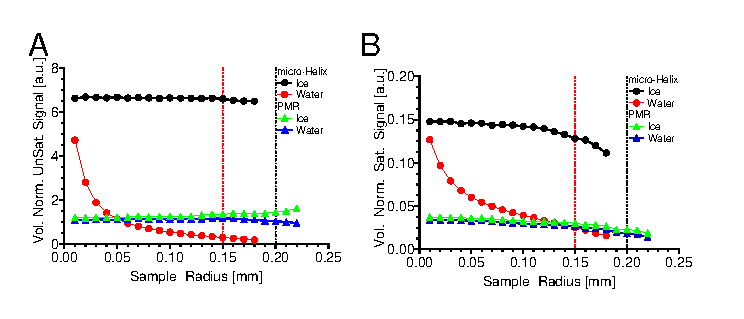
\includegraphics[width=\textwidth]{Kapitel/Ch2-Images/Ch2-AbsSweepOutputA.eps}
 \caption[Volume normalized swept EPR signal optimization.]{Volume normalized Swept EPR signal for the PMR with sapphire substrate (black; $\blacktriangle$) and the 0.4~mm micro-helix (red; $\CIRCLE$) with a water (solid) and ice (dashed) sample. Shown are the data from the A) unsaturated EPR signal and B) saturable EPR signal normalized to sample volume. The active region of the micro-helix and planar micro-resonator is assumed to be 1.2~mm and 1.1~mm, respectively. The dashed-dot line indicates the largest practical capillary inner radius for the helix (red) and PMR (black).}
 \label{fig:AbsSweptData}
\end{figure}

This example assumed the sample tube is filled and extends beyond the active region. It is noted that the active length of the two resonators is different and the data plotted in Fig.~\ref{fig:SweptData} can be normalized to the active volume and a comparison of the ``absolute sensitivity'' can be performed. Based on the magnetic field profile of  Figs.~\ref{ch2-fig:FieldData}E and \ref{ch2-fig:FieldData}F, the active region of the micro-helix and planar micro-resonator are assumed to be 1.2~mm and 1.1~mm, respectively, and a volume normalized signal is plotted in Fig.~\ref{fig:AbsSweptData}. 

At a fixed sample volume, the losses in the micro-helix associated with the aqueous sample still significantly affect the performance of the resonator.  Plotted in Figs.~\ref{fig:AbsSweptData}A and \ref{fig:AbsSweptData}B as a solid line for the micro-helix (red; $\CIRCLE$). However, compared to the PMR (black; $\blacktriangle$) there exists some sample volumes where the micro-helix yields a higher EPR signal. Finally, at a fixed sample volume and a relatively lossless sample, the micro-helix significantly outperforms the PMR geometry, plotted in Figs.~\ref{fig:AbsSweptData}A and \ref{fig:AbsSweptData}B as dashed lines.

These simulations demonstrate that the self-resonant micro-helix should be used primarily for frozen or lossless samples. However, for extremely small aqueous sample volumes (<9~nl), the micro-helix outperforms the PMRs. This is primarily due to the PMR planar geometry which limits the $Q$-value (50-180) and produces a strong inhomogeneity of the microwave magnetic field compared to the microwave magnetic field of the self-resonant micro-helix. 

\subsection{Experimental Comparison of Resonators.}
The PMRs were fabricated by printing the micro-resonator geometry on a substrate using photo\-/lithographic techniques. \cite{Suter2005, Suter2008, suter2015} PMRs show significant improvement in absolute spin sensitivity compared to the best commercial probeheads available. \cite{ ReijerseSavitsky2017} PMRs can be produced relatively cheaply using semiconductor etching techniques and laser scribing and configured for many frequencies with inner diameter sample sizes of 20-1000 $\mu$m. Furthermore, these structures offer excellent filling factors, high resonator efficiencies, and minimal power dissipation. It was recently demonstrated that a planar micro-resonators with Rogers RO6010LM substrate and a 500~$\mu$m sample diameter can be successfully employed for the study of crystals of inorganic metal complexes as well as [NiFe]-hydrogenase (0.35 $\times$ 0.2 $\times$ 0.2~mm$^3$) at 14~GHz, equipped with a specially designed cryogenic receiver at a temperature of 12~K. \cite{NARKOWICZ201379} Yet, such designs require a modified bridge to accommodate the cryogenic amplifier setup.

Improvement of the $Q$-value of the PMR geometry is reported here. By changing the substrate from Rogers RO6010LM substrate to single-crystal sapphire the $Q$-value increases by a factor of 3 and matches the simulations in Fig.~\ref{fig:AbsSweptData}B. The reduction of the $Q$-value using the Rogers RO6010LM substrate is not just the loss tangent of the material but partially due to surface roughness which gives rise to Ohmic losses.

The self-resonant micro-helix geometry wound around a 0.4~mm capillary is shown in Fig.~\ref{fig:fabricated}A. The final number of the micro-helix windings is determined by the pitch of the helix, the quartz capillary sample tube (0.4~mm outer diameter 0.3~mm inner diameter), and the surrounding Rexolite which all affect the resonance frequency. The fabricated 6.5-turn micro-helix had a resonant frequency around 9.7~GHz when coupled to the printed-circuit board inductive coupler. 

Simulated comparison of the fabricated micro-helix geometry with commercial (Bruker MD5W1 and Bruker MS3) and state-of-the-art (PMR; based on Rogers RO6010LM printed-circuit board or sapphire substrates) microwave probes is provided in Tables~\ref{table:signal} and \ref{table:chars}. Simulations were performed assuming a fixed sample geometry of 0.1~mm diameter by 0.1~mm height cylindrical sample. The simulated sample allows for absolute sensitivity comparisons amongst the resonator designs. 

\begin{table}[htb]
\centering
\caption[Resonator EPR signal characteristics calculated and measured.]{Resonator EPR signal characteristics calculated and measured for a fixed sample geometry.}
\label{table:signal}
\begin{tabular}{l|l|l|l|l}
 & \multicolumn{2}{l|}{UnSat. Signal} & \multicolumn{2}{l}{Sat. Signal}\\
Geometry & Calc. & Meas. & Calc. & Meas.\\ \hline \hline
Bruker MD5W1 & 1.0 & 1.0 & 1.0 & 1.0 \\ \hline
Bruker MS3 & 1.5 & 1.2 & 1.0 & 1.0 \\ \hline
PMR RO6010LM & 4.4 & 1.2 & 0.9 & 1.2 \\ \hline
PMR Sapphire & 18.6 & 13.3 & 3.9 & 3.8 \\ \hline
Micro-Helix & 35.7 & 28.2 & 6.1 & 5.7 \\
\end{tabular}
\end{table}

\begin{table}[htb]
\centering
\caption[Resonator characteristics calculated and measured.]{Resonator characteristics calculated and measured.}
\label{table:chars}
\begin{tabular}{l|c|c|c|c|c}
\multicolumn{1}{l}{} & DR & LGR & \multicolumn{2}{c|}{PMR} &  \\
\multicolumn{1}{c||}{Geometry} & MD5W1 & MS3 & 6010LM & Sapphire & Micro-Helix \\ \hline \hline
\multicolumn{1}{l||}{Freq. Calc.} & \multicolumn{1}{c|}{9.67} & \multicolumn{1}{c|}{9.67} & \multicolumn{1}{c|}{9.87} & \multicolumn{1}{c|}{9.87} & 9.78 \\ \hline 
\multicolumn{1}{l||}{Freq. Meas.} & \multicolumn{1}{c|}{9.69} & \multicolumn{1}{c|}{9.69} & \multicolumn{1}{c|}{9.58} & \multicolumn{1}{c|}{9.58} & 9.73 \\ \hline 
\multicolumn{1}{l||}{$Q_0$-value Calc.} & \multicolumn{1}{c|}{8860} & \multicolumn{1}{c|}{870} & \multicolumn{1}{c|}{90} & \multicolumn{1}{c|}{190} & 360 \\ \hline 
\multicolumn{1}{l||}{$Q_0$-value Meas.} & \multicolumn{1}{c|}{6650} & \multicolumn{1}{c|}{600} & \multicolumn{1}{c|}{61} & \multicolumn{1}{c|}{181} & 220 \\ \hline
\multicolumn{1}{l||}{$\Lambda$ Calc. {[}mT/W$^{1/2}${]}} & \multicolumn{1}{c|}{0.60} & \multicolumn{1}{c|}{0.68} & \multicolumn{1}{c|}{1.9} & \multicolumn{1}{c|}{2.9} & 4.1 \\ \hline 
\multicolumn{1}{l||}{$\Lambda_{ave}$ Calc. {[}mT/W$^{1/2}${]}} & \multicolumn{1}{c|}{0.60} & \multicolumn{1}{c|}{0.68} & \multicolumn{1}{c|}{1.5} & \multicolumn{1}{c|}{2.6} & 4.0 \\ \hline 
\multicolumn{1}{l||}{P$_{1/2}$ Meas. {[}mW{]}} & \multicolumn{1}{c|}{19.2} & \multicolumn{1}{c|}{18.4} & \multicolumn{1}{c|}{17.3} & \multicolumn{1}{c|}{1.8} & 0.8 \\ \hline 
\multicolumn{1}{l||}{$\Lambda_{ave}$ Meas. {[}mT/W$^{1/2}${]}} & \multicolumn{1}{c|}{–} & \multicolumn{1}{c|}{–} & \multicolumn{1}{c|}{–} & \multicolumn{1}{c|}{2.2} & 3.2
\end{tabular}
\end{table}

\paragraph{Power Saturation Measurements in All Resonators}
Experimentally, a minuscule amount of lithium phthalocyanine (LiPC)\cite{Liu5438} is embedded in Crytoseal (or similar) wax and is used as a point sample. The LiPC sample produces a very sharp line width (less than 0.05~mT) in the presence of oxygen (narrower without oxygen present), saturates at large values of ${\mathbf H}_{1r}$, and one needs very little sample volume to observe the signal. Therefore the use of LiPC allows for a fair comparison between all resonators by using the same sample throughout the experiments.\footnote{The term ``minuscule'' is defined as enough sample to observe a signal in the Bruker MD5W1 without causing line broadening in the micro-helix geometry. Such line broadening is due to a radiation dampening-like behavior caused by the large filling factor $\eta$.}

Power saturation experiments that were performed with the LiPC sample are plotted in Fig.~\ref{fig:lipcpwrsat}. From the power saturation data, EPR characteristics for each resonator can be ascertained and tabulated in Tables~\ref{table:signal} and \ref{table:chars}. The unsaturable signal is measured at constant microwave power (0.01~mW), while the saturable signal is measured at the power where the EPR signal amplitude is maximum (P$_{1/2}$-value; indicated by $\Diamond$). At the P$_{1/2}$-value, the B$_{1r}$ incident on the sample is identical in each of the resonators. For the power saturation experiments used in this work, the microwave power was stepped in 3~dB increments from 200~mW to 0.2~$\mu$W (0-60~dB). Each scan was 30~s over 1~mT with 4096 pts, receiver gain of 60~dB and 100~kHz field modulation at 0.1~mT in all resonators. The over-modulation of the LiPC sample was used to increase the sensitivity in the Bruker commercial resonators while increasing the intrinsic line width (line-height--line-width compromise, discussed in Ref.~[5.\kern-0.4em\citenum{eaton2010quantitative}]). 

\begin{figure}[htb]
\centering
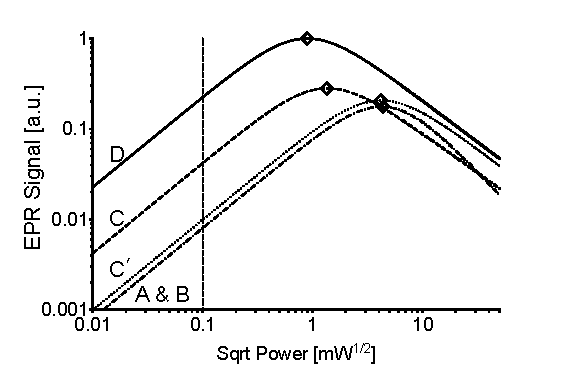
\includegraphics{Kapitel/Appendix/Images/S4-LiPCPowerSat.eps}
\caption[Power saturation data of LiPC comparing resonators.]{Power saturation data of LiPC showing the A) Bruker MD5 (dash-dot), and B) Bruker MS3, $\Omega$-type PMR with 0.5~mm sample loop with C) sapphire substrate (dashed) and C$'$) Rogers 6010LM substrate (dotted), and D) micro-helix (solid). EPR saturable signal is taken at peak signal (P$_{1/2}$-value, constant microwave field; indicated by $\Diamond$), while EPR unsaturable signal is taken at 0.01~mW (constant microwave power; dotted line).}
\label{fig:lipcpwrsat}
\end{figure}

As described in Table~\ref{table:signal}, if the EPR signal cannot be saturated (UnSat.; Eqn.~\ref{ch2-eq:su}) a factor of approximately 28 can be achieved compared to commercially available probeheads. EPR signals that cannot be saturated are proportional to the square root of the incident microwave power and, therefore, the EPR signal intensity is only limited by the amount of power available. However, most protein samples saturate readily, and, as such, the maximum signal that can be obtained is determined by the microwave magnetic field at the sample. When the sample is saturable (Sat.; Eqn.~\ref{ch2-eq:ss}), a factor of 5.7 can be achieved. The micro-helix exhibits the highest absolute sensitivity with no modification to the commercial bridge. 

The ratio of two P$_{1/2}$-values can be compared to the square of the ratio of $\Lambda_{ave}$. The data for the Bruker MS3 and MD5W1, in our hands, lay on top of each other for the LiPC point sample.

\paragraph{Measurement of $\Lambda_{ave}$ in the PMR and micro-Helix}
In order to measure the B$_{1r}$ directly, a series of pulse nutation experiments were performed. \cite{schweiger2001principles} The pulse nutation experiments were performed with an echo detected EPR signal using a 40~ns $\pi$/2 pulse and a pulse separation of 300~ns. An HA6047 300~W amplifier (HBH Microwave GmbH, Stutensee, DE) was used for all resonators and the power attenuation was adjusted for a maximum echo. From the nutation experiment oscillations, one can use Eqn.~\ref{eqB1rrab} and solve for B$_{1r}$ in Gauss and $f_{rab}$ is equal to the inverse of the time in seconds for a whole ($2\pi$) oscillation. The value of B$_{1r}$ is converted to mT (divide by 10) and normalized to the incident power by,
\begin{equation}
\Lambda_{ave} = \frac{B_{1r}}{(P/2^{\zeta/3})^{1/2}}\qquad [\text{mT/W}^{1/2}],
\end{equation}
where $P$ is the maximum power available (in this case, 300~W) and $\zeta$ is the attenuation of that power set on the console in dB. 

The sample was a 2\% w/w BDPA ($\alpha$,$\gamma$-bisdiphenylene-$\beta$-phenylallyl; Sigma-Aldrich Chemicals; CAS number 35585-94-5) in polystyrene and, in our laboratory, is used as a pulse EPR standard. The PS and BDPA are fully dissolved in toluene, laid out onto a covered Pyrex Petri dish, and left to evaporate for several days. The sample is then cut and placed in the sample tube for further testing. For direct measurement of $\Lambda_{ave}$, an EPR nutation experiment was performed at three pulse powers using the 2\% w/w BDPA in polystyrene and cut to 0.55 $\times$ 0.18 $\times$ 0.08~mm$^3$. The micro-helix has a measured power conversion efficiency parameter of 3.2~mT/W$^{1/2}$ which corresponds, for an $S=1/2$ spin system with a $g$-value of 2, to a $\pi/2$ pulse of 20~ns with an incident power of only 20~mW. No signal was measurable in the PMR RO6010LM, MS3, and MD5W1 due to a lack of sensitivity. However, the PMR with a sapphire substrate has a good efficiency parameter of 2.2~mT/W$^{1/2}$ which corresponds, for an $S=1/2$ spin system with a $g$-value of 2, to a $\pi/2$ pulse of 20~ns with an incident power of approximately 40~mW. These data are tabulated in Table~\ref{table:chars}.

\subsection{EPR of Photosystem II tyrosine D radical}
In the previous section, it has been shown that the self-resonant micro-helix outperforms both the commercial resonators and state-of-the-art PMR resonators in EPR experiments with standard samples. To further benchmark the micro-helix geometry a protein sample, specifically, photosystem II is measured. In photosystem II, water oxidation takes place at the tetranuclear manganese cluster, with a redox-active tyrosine radical (Y$_Z^\bullet$) as an interface to the light-induced electron transfer process, \cite{Lubitz2019} shown in Fig.~\ref{fig:psiicore}.\footnote{\label{CCnotRef} Ref.~[5.\kern-0.4em\citenum{Lubitz2019}] is distributed under the terms of the Creative Commons Attribution 4.0 International License (\textit{http://creativecommons.org/licenses/by/4.0/)}} Symmetrically to Y$_Z^\bullet$, a long-lived tyrosine radical (Y$_D^\bullet$) exists in the second branch of the photosystem II which contains no manganese cluster. In this work, the Y$_D^\bullet$ radical is used as a standard probe because it is stable for several hours under ambient conditions\cite{Saito7690} and has been well-characterized using a variety of EPR techniques. \cite{Hofbauer6623, STYRING201276} The hyperfine interactions from several protons, both on the phenyl ring and distal CH$_2$ carbon, lead to the distinct splittings of the radical (S=1/2). To generate the tyrosine radical (Y$_D^\bullet$) EPR signal, the photosystem II core complex samples are illuminated in ambient light and rapidly frozen. 

\begin{figure}[htb]
\centering
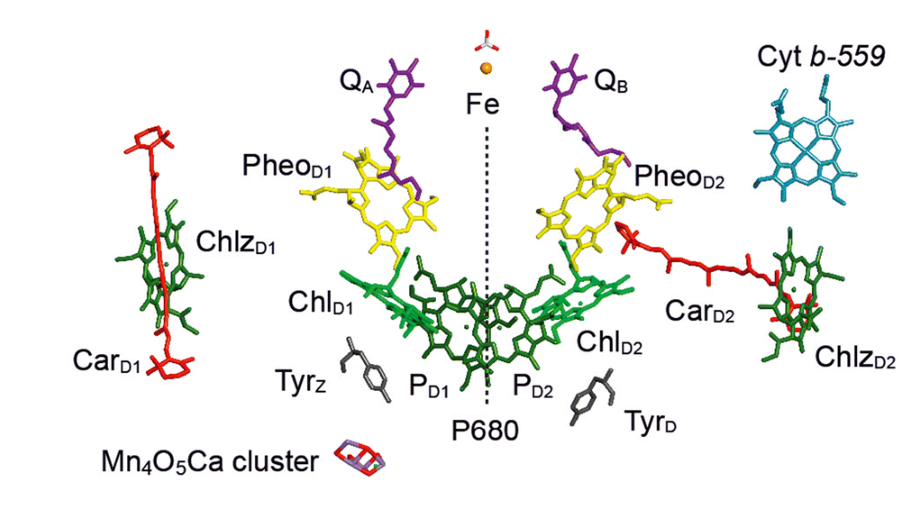
\includegraphics[width=0.8\textwidth]{Kapitel/Ch5-Images/PSII_CORE.eps}
\caption[Photosystem II core complex.]{Photosystem II core complex. The figure is modified from Ref.~[5.\kern-0.4em\citenum{Lubitz2019}] and reproduced with permission.$^3$}
\label{fig:psiicore}
\end{figure}

The tyrosine D radical (Y$_D^\bullet$) of photosystem II is measured in two forms: (i) a frozen solution sample of photosystem II (BBY particles) \cite{BBY1981} placed in a 0.3~mm inner diameter capillary and (ii) a 0.3 $\times$ 0.18 $\times$ 0.18~mm$^3$ single crystal of photosystem II core complexes. \cite{KERN2005147} In both photosystem II samples, the Y$_D^\bullet$ and first ligand-sphere are known to be identical. These samples provide a benchmark for future work.

\paragraph{Frozen solution EPR of Photosystem II tyrosine D radical (Y$_D^\bullet$).}
Shown in Fig.~\ref{fig:BBYPSII} is the Y$_D^\bullet$ radical EPR signal in an 85~nl frozen solution from photosystem II (BBY particles) at a temperature of 80~K using the self-resonant micro-helix. A continuous-wave EPR experiment, shown in Fig.~\ref{fig:BBYPSII}A, was performed on an Elexsys E580 X-band bridge by sweeping 10~mT in 1 minute (4096 points) with a modulation rate of 100~kHz and an amplitude of 0.5~mT. The data was averaged 49 times for a total of 49 minutes at an incident power of 0.2~$\mu$W. To further improve the signal-to-noise ratio of the continuous-wave experiment, a field-swept non-adiabatic rapid scan (NARS) experiment was performed, data are shown in Fig.~\ref{fig:BBYPSII}B. The field-swept non-adiabatic rapid scan (NARS) experiment was performed on the same commercial hardware using the rapid-scan method of M\"{o}ser {\em et al.}\cite{MOSER2017} and processed with the method described in Hyde {\em et al.}\cite{Hyde2013MDIFF} Herein, the scan rate was a sinusoidal 100~kHz field-sweep at 1~mT amplitude and a field-step size of 0.05~mT. The collected real and imaginary, pure-absorption and pure-dispersion, spectra were pseudo-modulated with a 0.5~mT moving difference (MDIFF)\cite{Hyde2013MDIFF} to compare to the field-modulated continuous-wave experiment. A factor of 2 in signal-to-noise improvement is obtained for the same signal acquisition time. 

\begin{figure}[htb]
\centering
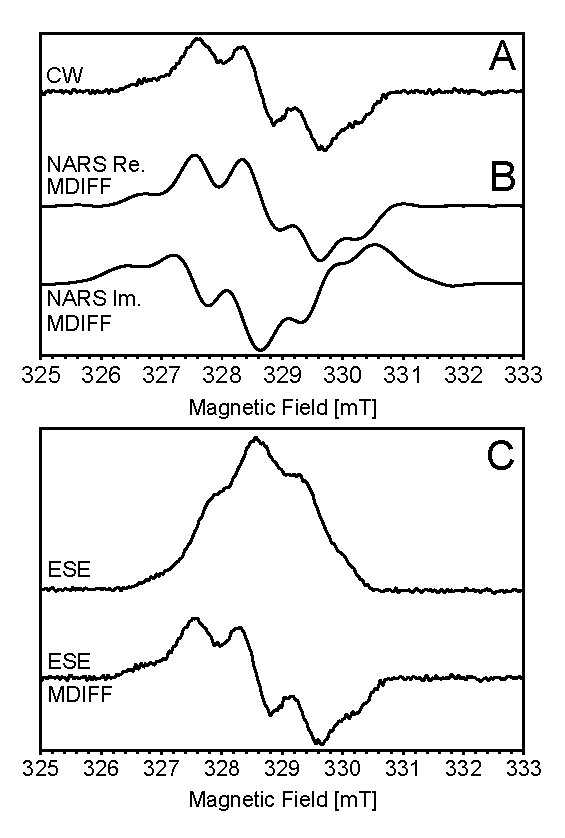
\includegraphics{Kapitel/Ch4-Images/02-PSII-BBY-Data.eps}
\caption[Frozen solution EPR on an 85~nl volume sample at X-band.]{Three frozen solution experiments with Y$_D^\bullet$ in photosystem II at 80~K were performed: A) continuous-wave, B) real and imaginary NARS, and C) ESE experiments. Calculated moving difference (MDIFF) pseudo-modulation of 0.5~mT is shown for the NARS and field-swept ESE experiments to directly compare to the continuous-wave EPR experiment.}
\label{fig:BBYPSII}
\end{figure}

A field-swept two-pulse electron spin-echo (ESE) EPR experiment was performed on the same commercial hardware over an 8~mT sweep, shown in Fig.~\ref{fig:BBYPSII}C. The field-swept ESE data was pseudo-modulated with a 0.5~mT MDIFF to compare the experiment with the field-modulated continuous-wave experiment of Fig.~\ref{fig:BBYPSII}A. The signal-to-noise ratio for all three experiments was calculated and tabulated in Table~\ref{table:snrcalc}. 

\begin{table}[htb]
\centering
\caption[Signal-to-noise calculations.]{Signal-to-noise calculations for the three experiments performed on the photosystem II Y$_D^\bullet$ radical in frozen solution at a temperature of 80~K. Approximately 1.6$\times10^{12}$ spins were calculated to be in the 85~nl that fill the micro-helix.}
\begin{tabular}{llll}
\multicolumn{1}{l|}{Experiment} & \multicolumn{1}{l|}{SNR Re.} & \multicolumn{1}{l|}{SNR Im.} & Time\\ \hline\hline
\multicolumn{1}{l|}{Continuous Wave} & \multicolumn{1}{c|}{197} & \multicolumn{1}{c|}{131} & \multicolumn{1}{c}{49~min} \\\hline
\multicolumn{1}{l|}{NARS} & \multicolumn{1}{c|}{4400} & \multicolumn{1}{c|}{2300} & \multicolumn{1}{c}{55~min} \\\hline
\multicolumn{1}{l|}{NARS (MDIFF)} & \multicolumn{1}{c|}{410} & \multicolumn{1}{c|}{423} & \multicolumn{1}{c}{--} \\\hline
\multicolumn{1}{l|}{ESE} & \multicolumn{1}{c|}{248} & \multicolumn{1}{c|}{--} & \multicolumn{1}{c}{45~min} \\\hline
\multicolumn{1}{l|}{ESE (MDIFF)} & \multicolumn{1}{c|}{106} & \multicolumn{1}{c|}{--} & \multicolumn{1}{c}{--}\\
\end{tabular}\label{table:snrcalc}
\end{table}

\begin{figure}[htb]
\centering
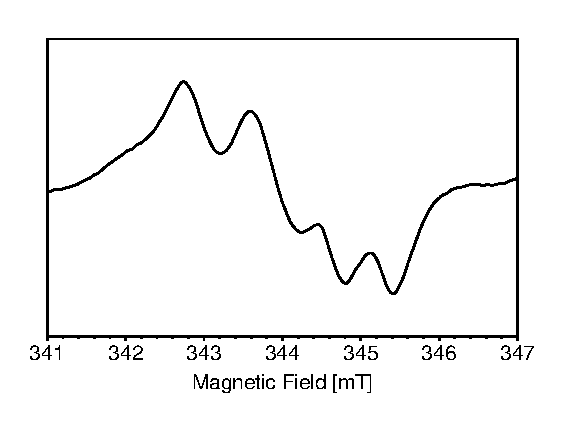
\includegraphics{Kapitel/Appendix/Images/S5-BBYMD5.eps}
\caption[CW EPR of frozen solution photosystem II in the Bruker MD5W1.]{Continuous-wave EPR of frozen solution photosystem II sample performed in the Bruker MD5W1 dielectric resonator at a temperature of 80~K. A signal-to-noise ratio of approximately 300 is calculated for a sample volume of 636~nl.}
\label{fig:BBYMD5}
\end{figure}

Finally, a comparison between the MD5W1 dielectric resonator and the self-resonant micro-helix was performed with the frozen solution photosystem II (BBY particle) sample at a temperature of 80~K. A continuous-wave EPR experiment was performed to compare the EPR signal obtained with 85~nl volume in the micro-helix. The photosystem II sample was placed in a 0.3~mm inner diameter quartz tube with a sample height of 9~mm (636~nl) and centered in the dielectric cavity. A signal-to-noise ratio of approximately 300 is calculated for a sample volume of 636~nl, shown in Fig.~\ref{fig:BBYMD5}. The spectrum was collected by sweeping 10~mT in 1 minute (4096 points) with a modulation rate of 100~kHz and an amplitude of 0.5~mT. The data are averaged 49 times for a total time of 49 minutes at an incident power of 3.1~$\mu$W. This power was chosen to compare the two samples at approximately the same B$_{1r}$ incident on the sample. Normalizing the signal-to-noise ratio with the volume yields a factor of approximately 5 improvement in absolute spin sensitivity using the self-resonant micro-helix compared to the MD5W1. These experiments serve to show the versatility of the micro-helix to perform EPR experiments on limited sample volumes (less than 85~nl) at X-band frequencies.

\paragraph{Single-Crystal continuous-wave EPR of the tyrosine D radical (Y$_D^\bullet$) in the photosystem II core complex.}
Shown in Fig.~\ref{fig:xTalPSII} is continuous-wave EPR data collected at two separate angles of the photosystem II Y$_D^\bullet$ radical in a single crystal at a temperature of 80~K as a sensitivity test for the 0.4~mm inner diameter self-resonant micro-helix. The photosystem II core complex crystal had a volume of 0.3 $\times$ 0.18 $\times$ 0.18~mm$^3$. The spectra were collected by sweeping 15~mT in 1 minute (4096 points) with a modulation rate of 100~kHz and an amplitude of 0.3~mT. The data were averaged 49 times for a total time of 49 minutes at an incident power of 0.2~$\mu$W. Simulations using the known $g$-tensor and hyperfine tensors \cite{Hofbauer6623} were performed with an Easyspin (http://easyspin.org; Ref.~[5.\kern-0.4em\citenum{STOLL200642}]) global fit routine to find the crystal orientation and plotted in red in Fig.~\ref{fig:xTalPSII}. At X-band, the g-anisotropy of the Y$_D^\bullet$ radical is very small and is not resolved. Instead, the orientation dependence is primarily determined by the hyperfine interaction pattern of the coupled proton nuclei. \cite{Hofbauer6623} Using only two angles, a unique fit cannot be found, but a demonstration of the Y$_D^\bullet$ features are shown. A non-specifically bound Mn$^{2+}$ signal was also present in the crystal, yielding the signals indicated by an asterisk (\mbox{\large $\ast$}). 

\begin{figure}[htb]
\centering
 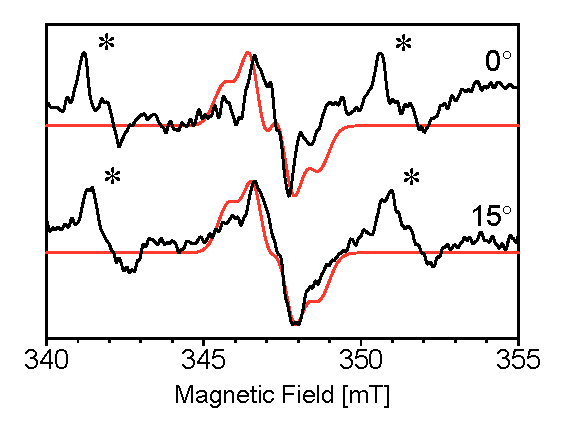
\includegraphics{Kapitel/Ch4-Images/03-PSII-xTal-Data.eps}
 \caption[Single-Crystal CW EPR of Y$_D^\bullet$ in the photosystem II core complex.]{Single-Crystal continuous-wave EPR of Y$_D^\bullet$ in photosystem II core complex. Continuous-wave EPR collected with the 0.4~mm inner diameter self-resonant micro-helix at two angles of the photosystem II Y$_D^\bullet$ radical from a single crystal at a temperature of 80~K. The crystal size was 0.3 $\times$ 0.18 $\times$ 0.18~mm$^3$. Shown in red is a fitted simulation with similar features. A non-specifically bound Mn$^{2+}$ signal is also present in the mother-liquor of the crystal, indicated by an asterisk (\mbox{\large $\ast$}). Each spectrum was collected in 49 minutes with a signal-to-noise ratio of approximately 35.}
 \label{fig:xTalPSII}
\end{figure}

The use of photosystem II crystals as a benchmark provides a challenging system to measure. The photosystem II core complex has a molecular weight of approximately 455~kDa as a monomer and each complex contains only one Y$_D^\bullet$ radical. Approximately 8.9$\times10^{12}$ Y$_D^\bullet$ radicals were present in the sample with a crystal size of 0.3 $\times$ 0.18 $\times$ 0.18~mm$^3$ and the crystal space group P${2_1\,2_1\,2_1}$. These data demonstrate the versatility of the micro-helix to study large complexes in small crystal dimensions. A photosystem II core complex crystal can be routinely grown to dimensions of 0.3~mm but requires significant effort to increase in size. Finally, the Y$_D^\bullet$ radical is easily saturable with large microwave magnetic fields, which limits the available microwave power and maximum EPR signal at a given temperature. Despite these challenges, a signal-to-noise of approximately 35 was calculated for the Y$_D^\bullet$ radical in the single-crystal sample. 

\paragraph{Qualitative Sensitivity Comparison of the X-band micro-helix to High-frequency single-mode resonators.}
Simulations were performed in Ansys HFSS comparing a cylindrical TE$_{011}$ cavity at W-band frequencies (95~GHz) to the micro-helix geometry at X-band frequencies using an 85~nl frozen solution sample. Assuming no g-anisotropy, the W-band TE$_{011}$ exhibits a factor of approximately 3 in improved EPR signal intensity compared to the micro-helix geometry at X-band frequencies. However, for example, the g-anisotropy at W-band spreads the tyrosine D radical in the photosystem II spectrum by a factor of 2 (see Fig.~2 in Ref.~[5.\kern-0.4em\citenum{Hofbauer6623}]); for some systems, the g-anisotropy may be more severe. Therefore, the micro-helix EPR sensitivity at X-band is comparable to a standard W-band system with a cylindrical TE$_{011}$ cavity. 

As the frequency becomes even higher, the resonator efficiency decreases due to losses on the surface of the resonator. For example, the Bruker 263~GHz single-mode resonator has a reported $\Lambda_{ave}$-value of 0.7 mT/W$^{1/2}$. \cite{bruker263} This is approximately half of the cylindrical TE$_{011}$ cavity at W-band. The lower $\Lambda_{ave}$ leads to only a factor of five in EPR signal improvement compared to the micro-helix at X-band. However, g-anisotropy becomes more severe as the operating frequency increases.

Therefore, the micro-helix geometry opens up the possibility to perform multi\-/frequency EPR on the same sample from X-band to 263~GHz. Using a 0.4~mm outer diameter capillary, a sample can be placed in the micro-helix at X-band and the same sample can then be inserted into a W-band or 263~GHz cavity. This ability allows for complementary techniques to be used for disentangling the angle dependencies of hyperfine-tensor interactions.


\section{Conclusions and Outlook}
An application of the self-resonant micro-helix geometry and planar-coupling structure that increases the EPR absolute spin sensitivity by a factor of approximately 30, if the signal is unsaturable, and 6, if the EPR signal can be saturated, was presented. For saturable EPR signals, such as those found in protein samples, the self-resonant micro-helix saves up to a factor of 32 in measuring time. From this gain of EPR sensitivity, the self-resonant micro-helix is well-suited for EPR studies on protein single-crystals with dimensions less than 0.3~mm. 

Due to the very high efficiency parameter of 3.2~mT/W$^{1/2}$, which corresponds to a $\pi/2$ pulse of 20~ns with an incident power of only 20~mW, the micro-helix geometry is advantageous in extending pulse EPR to experiments that usually require costly high-power microwave amplifiers (e.g. HYSCORE), further expanding the applicability of pulse EPR. This work also demonstrates that the self-resonant micro-helix performs well for field-swept non-adiabatic rapid scan (NARS) techniques due to its small size and ``open'' structure, which increases the continuous-wave EPR spin sensitivity further by a factor of 2 for the same experimental time. With a NARS experiment a the  self-resonant micro-helix is measured to have an absolute spin sensitivity of $63.5 \times 10^6$ Spins/G in 85~nl of sample for 50 minutes of collection time. Due to the relatively large bandwidth of the micro-helix (90~MHz critically-coupled), this geometry is particularly well-suited for frequency-swept NARS and rapid scan experiments which further improve the signal-to-noise ratio for saturable samples\cite{Hyde2013MDIFF, MOSER2017} and for the use of arbitrary-waveform generators for advanced pulse spectroscopy. \cite{schweiger2001principles, chirpedESEEM, goldfarb2018epr}

The micro-helix $Q$-value and high-efficiency parameter $\Lambda_{ave}$ significantly reduces the dead-time making the resonator suitable for experiments that record the onset of the EPR signal during pulses. For example, assuming a typical X-band bandwidth of 70~MHz and a $Q_0$-value of 1000, a $\beta$ of 6.5 is needed to over-couple the cavity to the desired bandwidth. By also assuming it takes 15-time constants (factor of 2 for voltage detection), the ring-down of the cavity can be calculated by
\begin{equation}
    15 \times \tau_c = 15 \times 2 \times Q / 2 \pi \nu,
\end{equation}
where $\nu$ is the frequency of interest. This produces a dead-time of 67~ns. For the micro-helix, with a critically-coupled measured $Q_0$-value of 220 the dead-time is 55~ns.\footnote{While critically-coupled, the signal-to-noise is improved by a $\sqrt{2}$ compared to an over-coupled cavity.} Assuming the micro-helix can be over-coupled by a $\beta$ of 6.5, this leads to a dead-time of 15~ns. However, compared to the Bruker MS3, the micro-helix would need a factor of 10 less power for the same B$_{1r}$, lowering the number of time constants needed.

As this technology matures, further improvements to enhance the sensitivity based on new fabrication techniques and choice of other materials will be explored. Not only does the increase in sensitivity save time in EPR data measurements, but it also reduces the need for the availability of, or necessity to, grow larger crystals. Overall, the self-resonant micro-helix provides the possibility to study catalytically-active proteins at crystal dimensions relevant to X-ray crystallography diffraction and, as such, is a significant advancement in the field of enzyme research. 

{\renewcommand{\bibsection}{\clearpage\section*{\bibname}\markboth{\bibname}{\bibname}}
\renewcommand{\bibname}{CHAPTER 5. REFERENCES}
\bibliographystyle{elsarticle-num}
\bibliography{Kapitel/Ch5-References}
}
